\documentclass[a4paper,twocolumn,superscriptaddress,11pt,accepted=2017-05-09]{quantumarticle}
\pdfoutput=1
\usepackage[utf8]{inputenc}
\usepackage[english]{babel}
\usepackage[T1]{fontenc}
\usepackage{amsmath}
\usepackage{hyperref}

\usepackage{tikz}
\usepackage{lipsum}

\newtheorem{theorem}{Theorem}

\begin{document}

\title{Template demonstrating the quantumarticle document class}

\author{Lídia del Rio}
\affiliation{Institute for Theoretical Physics, ETH Zurich, Switzerland}
\author{Christian Gogolin}
\email{latex@quantum-journal.org}
\homepage{http://quantum-journal.org}
\orcid{0000-0003-0290-4698}
\thanks{You can use the \texttt{\textbackslash{}email}, \texttt{\textbackslash{}homepage}, and \texttt{\textbackslash{}thanks} commands to add additional information for the preceding \texttt{\textbackslash{}author}. If applicable, this can also be used to indicate that a work has previously been published in conference proceedings.}
\affiliation{ICFO-Institut de Ciencies Fotoniques, The Barcelona Institute of Science and Technology, 08860 Castelldefels (Barcelona), Spain}
\author{Marcus Huber}
\affiliation{Institute for Quantum Optics \& Quantum Information (IQOQI), Austrian Academy of Sciences, Boltzmanngasse 3, Vienna A-1090, Austria}
\author{Christopher Granade}
\author{Johannes J. Meyer}
\orcid{0000-0003-1533-8015}
\maketitle

\begin{abstract}
  In the standard, \texttt{twocolumn}, layout the abstract is typeset as a bold face first paragraph.
  Quantum also supports a \texttt{onecolumn} layout with the abstract above the text.
  Both can be combined with the \texttt{titlepage} option to obtain a format with dedicated title and abstract pages that are not included in the page count.
  This format can be more suitable for long articles.
  The \texttt{abstract} environment can appear both before and after the \texttt{\textbackslash{}maketitle} command and calling \texttt{\textbackslash{}maketitle} is optional, as long as there is an \texttt{abstract}.
  Both \texttt{abstract} and \texttt{\textbackslash{}maketitle} however must be placed after all other \texttt{\textbackslash{}author}, \texttt{\textbackslash{}affiliation}, etc.\ commands, see also Section~\ref{sec:title-information}.
  If you provide the ORCID number of an author by using the \texttt{\textbackslash{}orcid} command, the author name becomes a link to their page on \href{http://orcid.org/}{orcid.org}. 
\end{abstract}

In the \texttt{twocolumn} layout and without the \texttt{titlepage} option a paragraph without a previous section title may directly follow the abstract.
In \texttt{onecolumn} format or with a dedicated \texttt{titlepage}, this should be avoided.

Note that clicking the title performs a search for that title on \href{http://quantum-journal.org}{quantum-journal.org}.
In this way readers can easily verify whether a work using the \texttt{quantumarticle} class was actually published in Quantum.
If you would like to use \texttt{quantumarticle} for manuscripts not yet accepted in Quantum, or not even intended for submission to Quantum, please use the \texttt{unpublished} option to switch off all Quantum related branding and the hyperlink in the title.
By default, this class also performs various checks to make sure the manuscript will compile well on the arXiv.
If you do not intend to submit your manuscript to Quantum or the arXiv, you can switch off these checks with the \texttt{noarxiv} option.
On the contrary, by giving the \texttt{accepted=YYYY-MM-DD} option, with \texttt{YYYY-MM-DD} the acceptance date, the note ``Accepted in Quantum YYYY-MM-DD, click title to verify'' can be added to the bottom of each page to clearly mark works that have been accepted in Quantum. 

\section{Figures}
\begin{figure}[t]
  \centering
  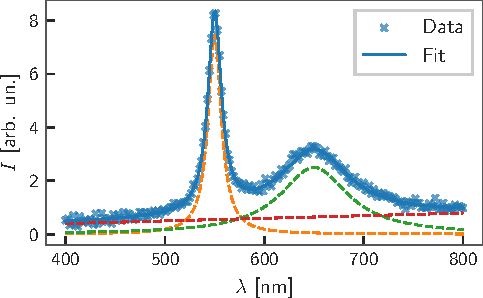
\includegraphics{example-plot.pdf}
  \caption{Every figure must have an informative caption and a number.
    The caption can be placed above, below, or to the side of the figure, as you see fit.
    The same applies for tables, boxes, and other floating elements. 
    Quantum provides a Jupyter notebook to create plots that integrate seamlessly with \texttt{quantumarticle}, described in Section \ref{sec:plots}.
    Figures spanning multiple columns can by typeset with the usual \texttt{figure*} environment.}
  \label{fig:figure1}
\end{figure}
See Fig.~\ref{fig:figure1} for an example of how to include figures.
Feel free to place them at the top or bottom of the page, or in the middle of a paragraph as you see fit.
Try to place them on the same page as the text referring to them.
A figure on the first page can help readers remember and recognize your work more easily.

\section{Sectioning and equations}
Sections, subsections, subsubsections, and paragraphs should be typeset with the standard LaTeX commands.
You can use the standard commands for equations.
\begin{align}
  \label{emc}
  E &= m\,c^2\\
  a^2 + b^2 &= c^2\\
  H\,|\psi\rangle &= E\,|\psi\rangle\\
  (\openone \otimes A)\,(B \otimes \openone) &= A \otimes B
\end{align}
For multi-line equations \texttt{align} is \href{http://tex.stackexchange.com/questions/196/eqnarray-vs-align}{preferable} over \texttt{eqnarray}.
Please refrain from using the latter.
For complex equations you may want to consider using the \texttt{IEEEeqnarray} environment from the \texttt{IEEEtrantools} package.
Whether you prefer to refer to equations as Eq.~\eqref{emc}, Equation~\ref{emc}, or just \eqref{emc} is up to you, but please be consistent and use the \texttt{\textbackslash{}eqref\{\dots\}} command instead of writing \texttt{(\textbackslash{}ref\{\dots\})}.
As a courtesy for your readers and referees, please suppress equation numbers only if there is a specific reason to do so, to not make it unnecessarily difficult to refer to individual results and steps in derivations.

\paragraph{Paragraphs}
The paragraph is the smallest unit of sectioning.
Feel free to end the paragraph title with a full stop if you find this appropriate.

\subsection{References and footnotes}
\label{sec:subsec1}
Footnotes\footnote{Only use footnotes when appropriate.} appear in the bottom of the page.
Please do not mix them with your references.

Citations to other works should appear in the References section at the end of the work.

\begin{theorem}[DOI links are required]
  Important: As Quantum is a member of Crossref, all references to works that have a DOI must be hyperlinked according to the DOI. Those links must start with \texttt{https://doi.org/} (preferred), or \texttt{http://dx.doi.org/}. Direct links to the website of the publisher are not sufficient.
\end{theorem}

This can be achieved in several ways, depending on how you are formatting your bibliography.
Suppose the DOI of an article \cite{examplecitation} that you want to cite is \texttt{10.22331/idonotexist}.
If you are formatting your bibliography manually, you can cite this work using the following in your \texttt{thebibliography} environment:
\begin{verbatim}
\bibitem{examplecitation}
  Name Surname,
  \href{https://doi.org/10.22331/
        idonotexist}{Quantum
        \textbf{123}, 123456 (1916).}
\end{verbatim}

\begin{theorem}[One citation per bibitem]
  Important: If you are formatting your bibliography manually, please do not group multiple citations into one \texttt{\textbackslash{}bibitem}.
  Having to search through multiple references to find the cited result makes your work less accessible for authors and grouping references can screw up our automatic extraction of citations.
\end{theorem}

We encourage the use of BibTeX to generate your bibliography from the BibTeX meta-data provided by publishers.
For DOI linking to work, the BibTeX file must contain the \texttt{doi} field as for example in:
\begin{verbatim}
@article{examplecitation,
  author = {Surname, Name},
  title = {Title},
  journal = {Quantum},
  volume = {123},
  page = {123456},
  year = {1916},
  doi = {10.22331/idonotexist},
}
\end{verbatim}
Several authors had problems because of Unicode characters in their BibTeX files.
Be advised that \href{http://wiki.lyx.org/BibTeX/Tips}{BibTeX does not support Unicode characters}.
All special characters must be input via their respective LaTeX commands.

If you are using BibTeX, you can load the \texttt{natbib} package by putting
\begin{verbatim}
\usepackage[numbers,sort&compress]{natbib}
\end{verbatim}
in the preamble of your document and then use the \texttt{plainnat} citation style by including your BibTeX bibliography \texttt{mybibliography.bib} where you want the bibliography to appear as follows:
\begin{verbatim}
\bibliographystyle{plainnat}
\bibliography{mybibliography}
\end{verbatim}
The quantumarticle class automatically detects that the \texttt{natbib} package was loaded and redefines the \texttt{\textbackslash{}doi} command to create hyperlinks.
This is likely the easiest option if you are converting from another document class.

If you want to use BibLaTeX, you can instead add
\begin{verbatim}
\usepackage[backend=bibtex]{biblatex}
\addbibresource{mybibliography.bib}
\end{verbatim}
to the preamble of your document and then output the bibliography with
\begin{verbatim}
\printbibliography
\end{verbatim}
where appropriate.
You then have to upload the .bbl file along with the other source files when submitting to the arXiv.
Due to incompatibilities between different LaTeX version we unfortunately cannot recommend this option \cite{biblatexsubmittingtothearxiv}.

The quantumarticle class automatically detects that the \texttt{biblatex} package was loaded, sets the default option \texttt{doi=true} to include the DOI in the bibliography, and declares a suitable field format to make it a hyperlink.
Due to issues with \texttt{biber} we recommend to use the \texttt{bibtex} backend of \texttt{biblatex}.

More information on how to get DOI links in your document can be found on StackExchange \cite{howtogetdoilinksinbibliography,automaticallyaddingdoifieldstoahandmadebibliography}.
Feel free to change the appearance of citations in any way you like by using a different \texttt{bibliographystyle} or via the advanced mechanisms provided by BibLaTeX.
The only two requirements are that citations must uniquely identify the cited work and that they must contain a DOI hyperlink whenever possible.

\begin{theorem}[Use \texttt{\textbackslash pdfoutput=1}]
  In order to get correct line breaks within hyperlinks and to make sure the arXiv produces a PDF as output, please add the line 
\begin{verbatim}
\pdfoutput=1
\end{verbatim}
  within the first 5 lines of your main LaTeX file, as suggested by the arXiv \cite{arxivpdfoutput}.
\end{theorem}

\section{Plots}
\label{sec:plots}
Quantum provides a \href{https://jupyter.org/}{Jupyter notebook} based on the widely used \href{https://matplotlib.org/}{matplotlib} library that greatly simplifies the creation of plots that integrate seamlessly with the \texttt{quantumarticle} document class. This is intended as a service to the authors, is \textit{not} mandatory, and currently in beta stage. You can download the \href{https://raw.githubusercontent.com/quantum-journal/quantum-journal/master/quantum-plots.ipynb}{quantum-plots.ipynb} notebook and accompanying \href{https://raw.githubusercontent.com/quantum-journal/quantum-journal/master/quantum-plots.mplstyle}{quantum-plots.mplstyle} file from the \href{https://github.com/quantum-journal/quantum-journal}{quantumarticle GitHub repository}. You only need to specify the font size and paper format that were passed as options to \texttt{quantumarticle} to get plots with fitting font sizes and dimensions.
We strongly encourage authors to use the vector based PDF format for plots.

\begin{theorem}[Be mindful of the colorblind]
  About 4\% of the worlds population are affected by some form of color vision deficiency or color blindness.
  Please make sure that your plots and figures can still be understood when printed in gray scale and avoid the simultaneous use of red and green, as the inability to distinguish these two colors is the most widespread form of color vision deficiency.
\end{theorem}

\section{Summary section}
Longer articles should include a section that, early on, explains the main results, their limitations, and assumptions.
This section can be used to, for example, present the main theorem, or provide a summary of the results for a wider audience.

\section{Extra packages}
Quantum encourages you to load the following extra packages:
\begin{verbatim}
\usepackage[utf8]{inputenc}
\usepackage[english]{babel}
\usepackage[T1]{fontenc}
\usepackage{amsmath}
\usepackage{hyperref}
\end{verbatim}
If you do not load the \texttt{hyperref} package, quantumarticle automatically loads it for you.
Packages that change font settings, such as \texttt{times} or \texttt{helvet} should be avoided.

\section{Wide equations}
Very wide equations can be shown expanding over both columns using the \texttt{widetext} environment.
In \texttt{onecolumn} mode, the \texttt{widetext} environment has no effect.
\begin{widetext}
  \begin{equation}
|\mathrm{AME}(n=6,q=5)\rangle=\sum_{i,j,k=0}^4 |i,j,k,i+j+k,i+2j+3k,i+3j+4k\rangle
  \end{equation}
\end{widetext}
To enable this feature in \texttt{twocolumn} mode, \texttt{quantumarticle} relies on the package \texttt{ltxgrid}.
Unfortunately this package has a bug that leads to a sub-optimal placement of extremely long footnotes.

\section{Title information}
\label{sec:title-information}
You can provide information on authors and affiliations in the common format also used by \texttt{revtex}:
\begin{verbatim}
\title{Title}
\author{Author 1}
\author{Author 2}
\affiliation{Affiliation 1}
\author{Author 3}
\affiliation{Affiliation 2}
\author{Author 4}
\affiliation{Affiliation 1}
\affiliation{Affiliation 3}
\end{verbatim}
In this example affiliation 1 will be associated with authors 1, 2, and 4, affiliation 2 with author 3 and affiliation 3 with author 4.
Repeated affiliations are automatically recognized and typeset in \texttt{superscriptaddress} style.
Alternatively you can use a format similar to that of the \texttt{authblk} package and the \texttt{elsarticle} document class to specify the same affiliation relations as follows:
\begin{verbatim}
\title{Title}
\author[1]{Author 1}
\author[1]{Author 2}
\author[2]{Author 3}
\author[1,3]{Author 4}
\affil[1]{Affiliation 1}
\affil[2]{Affiliation 1}
\affil[3]{Affiliation 1}
\end{verbatim}

\bibliographystyle{plain}
\begin{thebibliography}{9}
\bibitem{examplecitation}
  Name Surname,
  \href{https://doi.org/10.22331/
        idonotexist}{Quantum
        \textbf{123}, 123456 (1916).}

\bibitem{biblatexsubmittingtothearxiv}
  StackExchange discussion on \href{http://tex.stackexchange.com/questions/26990/biblatex-submitting-to-the-arxiv}{``Biblatex: submitting to the arXiv'' (2017-01-10)}

\bibitem{arxivpdfoutput}
  Help article published by the arXiv on \href{https://arxiv.org/help/submit_tex}{``Considerations for TeX Submissions'' (2017-01-10)}

\bibitem{howtogetdoilinksinbibliography}
  StackExchange discussion on \href{http://tex.stackexchange.com/questions/3802/how-to-get-doi-links-in-bibliography}{``How to get DOI links in bibliography'' (2016-11-18)}
  
\bibitem{automaticallyaddingdoifieldstoahandmadebibliography}
  StackExchange discussion on \href{http://tex.stackexchange.com/questions/6810/automatically-adding-doi-fields-to-a-hand-made-bibliography}{``Automatically adding DOI fields to a hand-made bibliography'' (2016-11-18)}
\end{thebibliography}



\onecolumn\newpage
\appendix

\section{First section of the appendix}
Quantum allows the usage of appendices.

\subsection{Subsection}
Ideally, the command \texttt{\textbackslash{}appendix} should be put before the appendices to get appropriate section numbering.
The appendices are then numbered alphabetically, with numeric (sub)subsection numbering.
Equations continue to be numbered sequentially.
\begin{equation}
  A \neq B
\end{equation}
You are free to change this in case it is more appropriate for your article, but a consistent and unambiguous numbering of sections and equations must be ensured.

If you want your appendices to appear in \texttt{onecolumn} mode but the rest of the document in \texttt{twocolumn} mode, you can insert the command \texttt{\textbackslash{}onecolumn\textbackslash{}newpage} before \texttt{\textbackslash{}appendix}.   

\section{Problems and Bugs}
In case you encounter problems using the quantumarticle class please analyze the error message carefully and look for help online; \href{http://tex.stackexchange.com/}{http://tex.stackexchange.com/} is an excellent resource.
If you cannot resolve a problem, please open a bug report in our bug-tracker under \href{https://github.com/quantum-journal/quantum-journal/issues}{https://github.com/quantum-journal/quantum-journal/issues}.
You can also contact us via email under \href{mailto:latex@quantum-journal.org}{latex@quantum-journal.org}, but it may take significantly longer to get a response.
In any case, we need the full source of a document that produces the problem and the log file showing the error to help you.

\end{document}
